% !TEX root = 0-main.tex
\chapter{Анализ задачи}
\label{cha:analysis}
\textbf{Постановка задачи:} Алгоритм Ли для поиска пути (гексагональная сетка) на равностороннем 
четырехстороннем (в виде паралелограмма) дискретном рабочем поле. Длина сторон рабочего поля может
 варьироваться в пределах [10;100]. Требуется реализовать указанный в теме алгоритм. При этом вывод 
 итоговых и промежуточных результатов должен быть реализованы в виде svg графики.
\section{Гексагональная сетка}
В основе гексагональной сетки (\textit{англ.} hexagon grid) лежит правильный шестиугольник (\textit{англ.} hexagon), 
внутренние углы которого равны $120 \degree$. На гексагональной сетке две параллельные стороны 
всех шестиугольников могут располагаться либо параллельно оси ординат, либо оси абсцисс. Возьмем 
первый вариант и выведем математические формулы, которые описывают гексагональную сетку и 
её элементы на равностороннем треугольном дискретном рабочем поле (\textit{РТДРП}).
\par
Прежде всего необходимо задать размерность шестиугольника $hexSize$.
Она определяет расстояние углов от центра фигуры. 
Размерность паралелограмма обозначим через $dimension$.

\begin{figure}
	\centering
	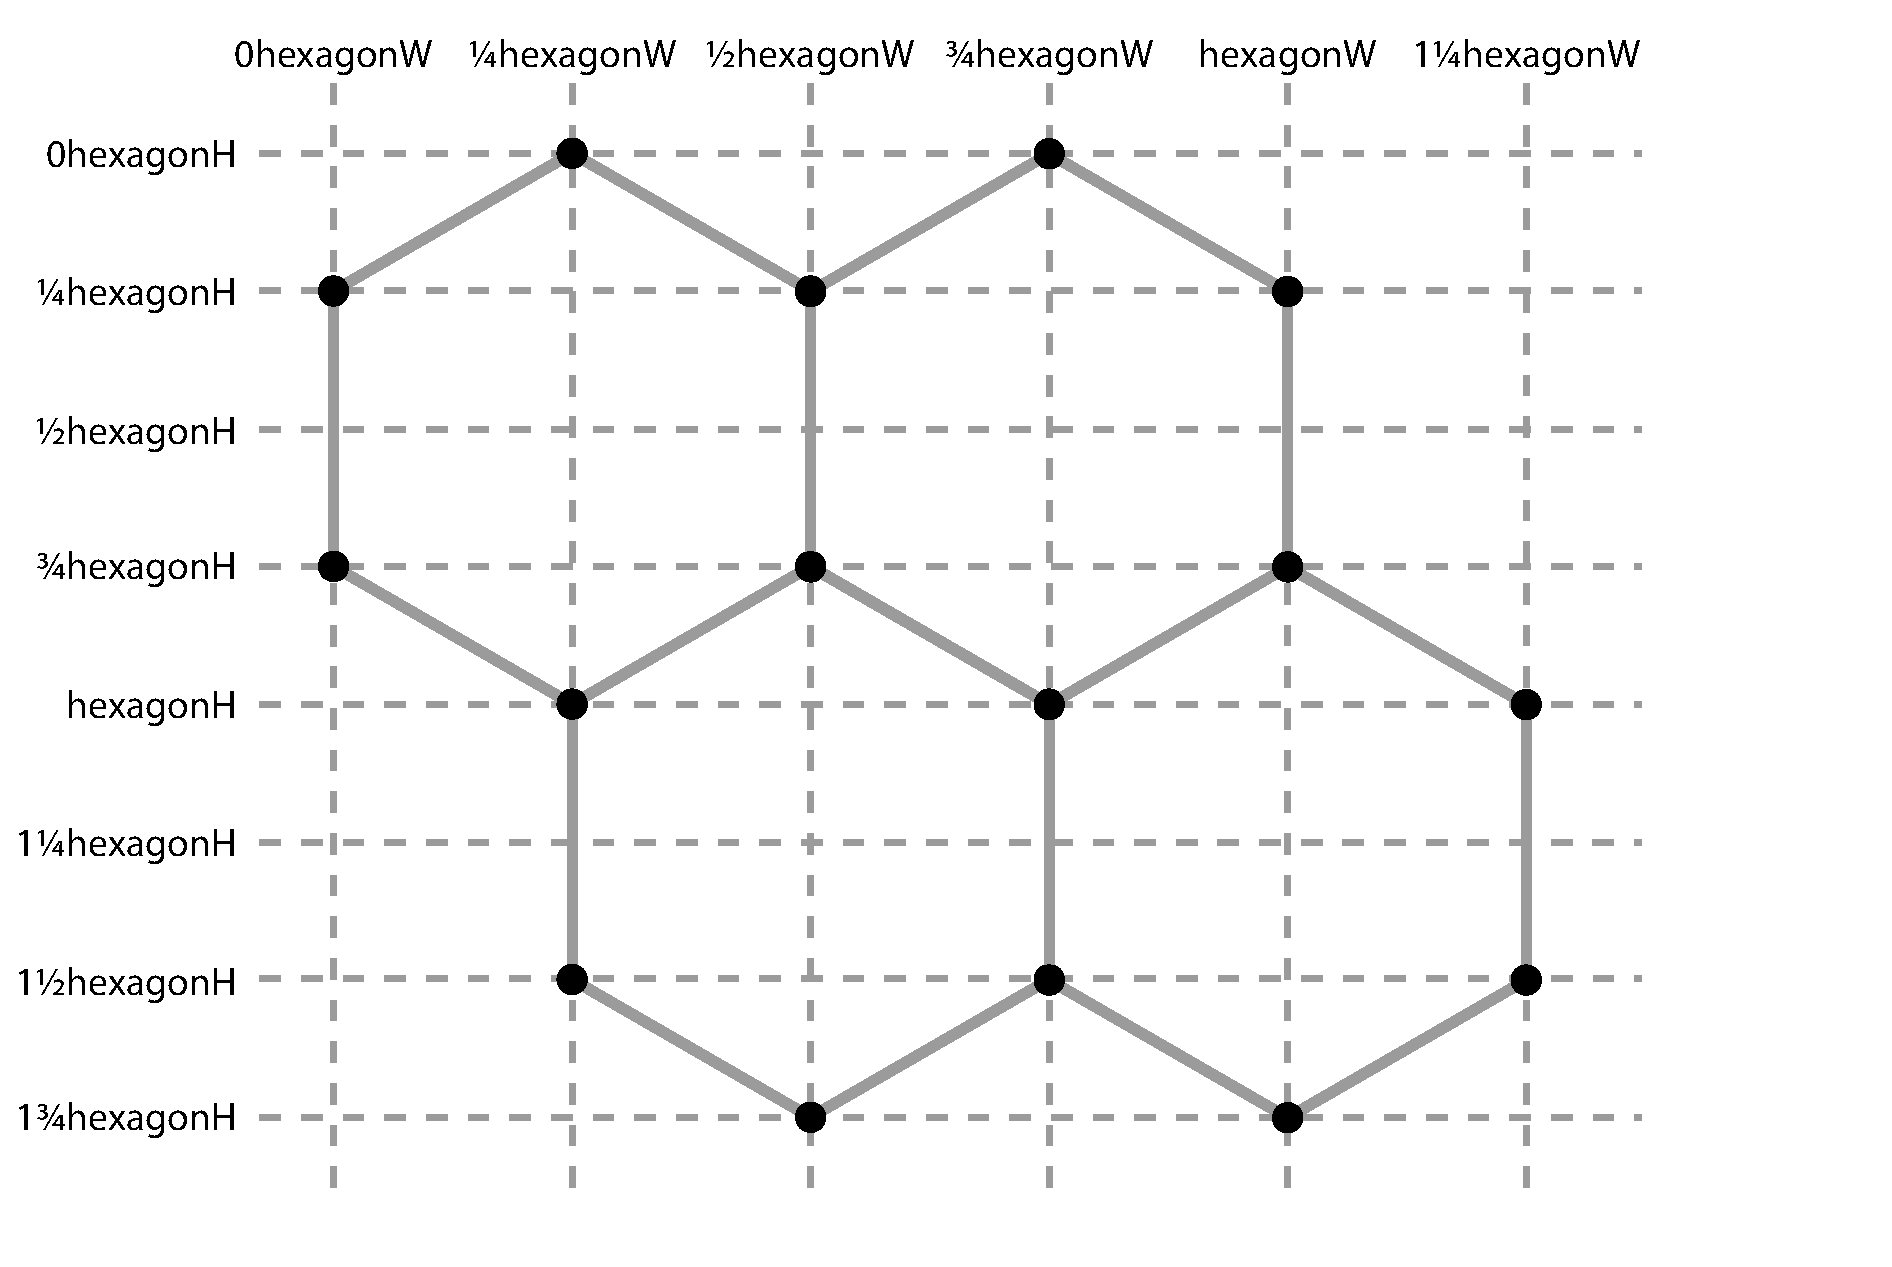
\includegraphics[height=0.35\textheight]{inc/img/hexagon_grid}
	\caption{Гексагональная сетка.}
	\label{analysis:hexagonGridWithPoints}
\end{figure}

Высота данного поля $gridHeight$ вычисляется по формуле: 
\begin{equation}
%\caption{Вычисление размера шестиугольника на основе ширины и высоты сетки.}
\label{hexGrid:gridHeight}
	gridHeight=hexH(\frac{3}{4}dimension+\frac{1}{4}),
\end{equation} 
где hexH --- высота шестиугольника, которую можно найти по формуле $2hexSize$. 
Ширина данного поля $gridWidth$ вычисляется по формуле: 
\begin{equation}
%\caption{Вычисление размера шестиугольника на основе ширины и высоты сетки.}
\label{hexGrid:gridWidth}
gridWidth=hexW\times dimension, 
\end{equation}
где hexW --- ширина 
шестиугольника, которая равна $hexSize\sqrt{3}$.

\section{Алгоритм Ли}
\label{analysis:li}

 \textbf{Алгоритм Ли} — волновой алгоритм поиска пути на карте, алгоритм трассировки. С его помощью можно построить путь, или трассу, между двумя любыми элементами в лабиринте. Из начального элемента распространяется в четырёх направлениях волна. Тот элемент, в который она пришла, образует фронт волны.

Элементы первого фронта волны являются источниками вторичных волн.

Элементы второго фронта генерируют волну третьего фронта и так далее. Процесс заканчивается тогда, когда достигается конечный элемент. На втором этапе строится трасса. Построение производится в соответствии с некоторыми правилами:
\begin{enumerate}

\item при построении трассы движение проходит в зависимости от выбранных приоритетов,
\item путевые координаты уменьшаются при переходе от начального элемента к конечному.
\end{enumerate}
Эти приоритеты выбираются в процессе разработки. В зависимости от выбора тех или иных приоритетов получаются различные трассы. Но в любом случае длина трассы остается одной и той же.

Используя волновой алгоритм, можно найти трассу в лабиринте с любым количеством стен. В этом и заключается \textbf{преимущество} его использования.

\textbf{Недостаток} алгоритма Ли заключается в том, что при построении трассы требуется большой объем памяти.






































